\chapter{Pilot Studies} \label{pilot_studies}

\section{Pre-pilot Study} \label{pre_pilot}
The pre-pilot was a very informal study aimed at assessing the functionality of the pseudo word-gesture keyboard implementation. This informal study was used to also test the conceptual feasibility of using 3-dimensions as a means of word separation for simulated touch input. See Chapter~\ref{keyboard_design} for more specific implementation details.

\subsection{Participants} \label{pre_participants}
A sample size of 2 was used in the pre-pilot study. Both participants were male, ages 24 and 25 and both participants had previous experience with gesture-controllers, touch screens, and word-gesture keyboards. Table~\ref{pre_participant_stats} provides the participants' information in detail.

\begin{table}[!b]
	\centering
	\caption[Pre-pilot Study Details of Participants]{\centering Participant information including age, gender, handedness, computer usage, and previous experiences.}
	\label{pre_participant_stats}
	\resizebox{\textwidth}{!}{\begin{tabular}{ c | c c c c c c c c c c}
		\hline
		\multirow{2}{*}{Subject} & \multirow{2}{*}{Gender} & \multirow{2}{*}{Age} & Computer Usage & \multirow{2}{*}{Handedness} & Hand Used & Touch-device & Gesture-controller & Word-gesturing & Impairment \\
		{} & {} & {} & per Week (hours) & {} & in Experiment & Experience & Experience & Experience & History \\
		\hline
		1 & m & 24 & 31 - 40 & right & right & yes & yes & yes & no \\
		2 & m & 25 & 50+ & right & right & yes & yes & yes & no \\
		\hline
	\end{tabular}}
\end{table}

\subsection{Input Devices and Interaction Styles}
The interaction methods used within the pre-pilot study were dependent on the currently active keyboard input forcing the user to only interact with one style of keyboard at a time. All of the keyboards were simulated on a 64-bit Windows 7 work station, with all receivers or controllers connected via USB 2.0. The participants were allowed to recalibrate the active keyboard's interaction plane at any time before starting the main task for a more comfortable experience. Calibration was only possible if applicable to the active keyboard input. Participants were also encouraged to reposition the gesture-controller to best fit their personal preference and were given the option to freely rest or raise their elbows during the experiment. More information about the implementation of specific keyboard interactions and calibrations can be found in Chapter~\ref{keyboard_design}. Every keyboard was designed for use by either right or left handed participants. Figure~\ref{fig_old_keyboard} shows the keyboard layout used for all keyboards other than the Xbox Controller keyboard, whereas Figure~\ref{fig_xbox_keyboard} shows the keyboard used for the Xbox Controller Keyboard.

\subsubsection{Leap Motion Static-air Keyboard}
The Leap Motion Static-air Keyboard used a Leap Motion controller which was placed on the desk in front of the participant. The participant then used a stylus which was tracked by the Leap Motion controller in order to interact with a projected interaction plane. A touch was simulated by the insertion of the stylus into the interaction plane and a release was simulated upon the removal of the stylus. The interaction plane could be calibrated at any time prior to the experiment.

\begin{figure}[h]
	\centering
	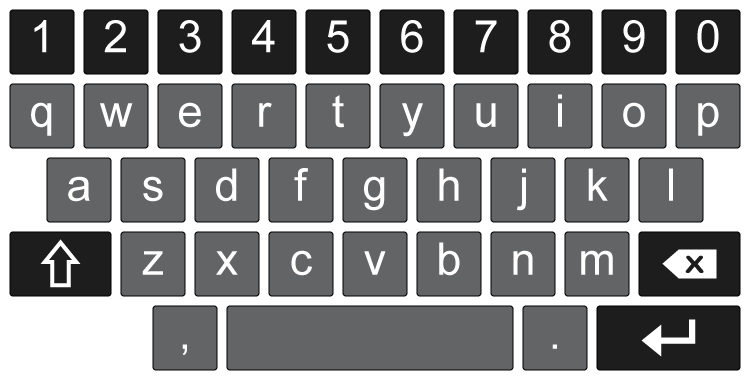
\includegraphics[width=6in]{Figures/fig_old_keyboard}
	\caption[Original Keyboard Layout]{The keyboard layout used during the pre-pilot study.}
	\label{fig_old_keyboard}
\end{figure}

\subsubsection{Leap Motion Pinch-air Keyboard}
The Leap Motion Pinch-air Keyboard also used a Leap Motion controller that was positioned on the desk in front of the participant. The participant then used their bare hand, which was tracked at the center of their palm, to interact with the projected interaction plane. Touch was simulated by having the participant make a pinching gesture with their hand and a release was simulated when the participant released the pinch, opening their hand again. As in the previous Static-air keyboard, the interaction plane could be calibrated at any time prior to the experiment.

\subsubsection{Leap Motion Surface Keyboard}
Again, for the Leap Motion Surface Keyboard, a Leap Motion controller was used for tracking. Unlike the Leap Static-air or Leap Pinch-air keyboards, the gesture controller was placed into a custom designed holder instead of on the desk in front of the participant. The holder was attached to an inclined surface with a printed keyboard fixed on top, as shown in Section~\ref{leap_surface}. Because identical placement was not guaranteed between uses, the Leap Motion Surface Keyboard required a single calibration after being inserted into the holder to accurately simulate an interaction plane projected onto the printed keyboard. The participant then used a stylus, as before, which was tracked by the Leap Motion controller in order to detect interaction. A touch was simulated by pressing the tip of the stylus against the printed keyboard and a release was simulated when the tip of the stylus was removed from the printed keyboard surface.

\subsubsection{Xbox Controller Keyboard}
The Xbox Controller Keyboard used an Xbox 360 Wireless Controller that transmitted information via the Microsoft Xbox 360 Wireless Receiver for Windows. The participants were required to use the directional sticks or the directional-pad in order to change which key was selected, and then used the `A' button in order to select the currently highlighted key. The Xbox Controller keyboard only allowed for single-input text entry, functioning in the same way as the default Xbox 360 virtual keyboard.

\begin{figure}[!t]
	\centering
	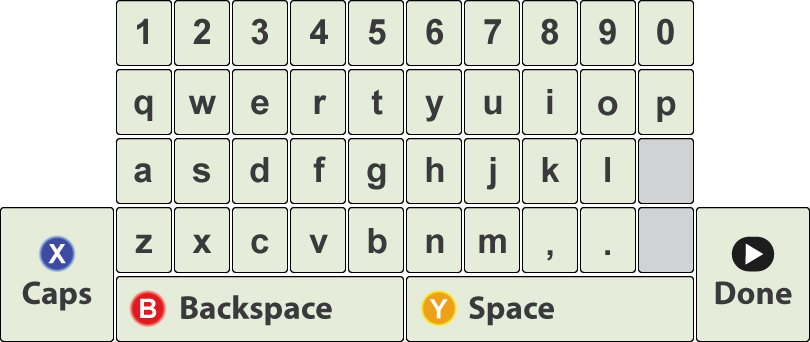
\includegraphics[width=6in]{Figures/fig_xbox_keyboard}
	\caption[Xbox Controller Keyboard Layout]{The keyboard layout used for the Xbox Controller Keyboard.}
	\label{fig_xbox_keyboard}
\end{figure}

\subsection{Task Design} \label{pre_task}
The design for the pre-pilot study included 4 different keyboard interaction styles representing each of the conditions that made up the task. The 4 conditions used were the Leap Motion Static-air, Leap Motion Pinch-air, Leap Motion Surface, and Xbox Controller keyboards.

The task consisted of 30 trials for each of the 4 keyboard interaction styles creating a total of 120 trials per participant. For each trial, a word of 3 to 6 characters in length was chosen at random from the Oxford English Dictionary and displayed on the screen. A blank text-area was positioned directly below the displayed word for the user-generated, transcribed text. Beneath both text areas, there was a virtual representation of the keyboard the participants were using. The participants were then required to use the currently active keyboard interaction style to enter the displayed word using word-gesturing. During the word-gesturing process, the participants were shown real-time updates to the displayed word and transcribed text as well as their movements within the virtual keyboard space. Detected key presses were appended directly to the transcribed text-area with correctly matching letters being colored green and text entry errors being colored red whereas only correctly matching letters were applied to the displayed word. The participants were required to use the active keyboard's backspace key to remove errors. Once a word was correctly entered, the participants were required to press the active keyboard's enter key to move on to the next word.

Small deviations in the above task were required for how the participants interacted with the Xbox Controller keyboard. For this keyboard, there was no word-gesturing feature implemented. Instead, the participant was asked to use single-input text entry using a standard Xbox 360 Controller. The Xbox Controller keyboard was implemented in the same way as a conventional console keyboard. The participants had to press the `A' button to select a letter, `Y' button to delete, and the `start' button to move to the next word.

\subsection{Experimental Design} \label{pre_experimental_design}
The initial pre-pilot study used a within-subjects design without any counterbalancing \cite{ref_within_subjects}. Both participants used every keyboard interaction style in a random order. The strength of a within-subjects design is the overall power increase and reduction in error variance associated with individual differences. The weakness of using the within-subjects design is that it suffers from ``carryover effects'' (the participation in one condition may affect performance in other conditions) between each keyboard interaction style.

\subsection{Procedure} \label{pre_procedure}
There was only a single study visit for each participant in which all tasks were performed. The study visit took between 30 and 45 minutes to complete depending on the number of calibrations. The full set of tasks and their expected durations are detailed in Table~\ref{pre_schedule_of_assessments}, the pre-pilot schedule of assessments. The participants followed the same process for each of the 4 keyboard interaction styles' tasks.

\begin{table}[!b]
	\centering
	\caption[Pre-pilot Study Schedule of Assessments]{\centering Schedule of Assessments for a single study visit during the pre-pilot study (in minutes).}
	\label{pre_schedule_of_assessments}
	\resizebox{\textwidth}{!}{\begin{tabular}{ l | c c c c c | c}
		\hline
		\multirow{2}{*}{Step} & \multirow{2}{*}{Controller} & Leap Motion & Leap Motion & Leap Motion & Exit & \multirow{2}{*}{Total}  \\
		{} & {} & Surface & Static-air & Pinch-air & Survey & {}  \\
		\hline
		explain & 0.5 & 0.5 & 0.5 & 0.5 & 0 & 2 \\
		practice & 5 & 5 & 5 & 5 & 0 & 20 \\
		calibrate & 0 & 2 & 2 & 2 & 0 & 6 \\
		task & 3 & 3 & 3 & 3 & 0 & 12 \\
		survey & 0 & 0 & 0 & 0 & 5 & 5 \\
		\hline
		Total & 8.5 & 10.5 & 10.5 & 10.5 & 5 & 45 \\
		\hline
	\end{tabular}}
\end{table}

First, the participants were given a brief verbal explanation and physical demonstration of the active keyboard input. The explanation dialog contained the name of the active keyboard and the method of interaction. The researcher then demonstrated how to enter the word ``test'' using the active keyboard. The participants were then given the stylus and control of interaction with the keyboard in order to become familiar with the interaction style.

Participants were then instructed to use the keyboard to perform practice words that were randomly chosen from the Oxford English Dictionary between 3 and 6 characters long. No practice words were duplicated and the dictionary was filtered for offensive words. There was no limit placed on how many words could be performed while practicing. The participants were told to continue until they felt they were able to efficiently and comfortably type each word with minimal errors. During the practice phase, the opportunity to optionally recalibrate the interaction-space any number of times was given if applicable to the active keyboard.

Next, the participants performed the task itself. As detailed in Section~\ref{pre_task}, the participants were instructed to enter a total of 30 words for the current keyboard interaction style. None of the experiment words were duplicated between themselves or the practice words and again were pulled at random from the Oxford English Dictionary between 3 and 6 characters, filtering for swear words. Participants were not allowed to recalibrate the interaction space during the task. 

After all tasks were completed for each of the 4 interaction styles, the participants were asked to fill out an exit survey. The exit survey asked the participants for their age, gender, major, and handedness as well as several questions detailing any prior touch, gesture-controller, or word-gesturing experience or impairments that might relate to the study. Finally, the participants were required to fill out the Likert scale relating to difficulty, discomfort, and fatigue experienced when using the interaction styles, as well as rank each interaction style on a numerical scale from best to worst.

\subsection{Dependent Measures}
The pre-pilot study collected qualitative testimonials alongside the exit survey. Participants were encouraged to give feedback of their experience during and after the experiment. The feedback was then used to refine the pseudo word-gesture keyboard implementation and assess the keyboard layout. Additionally, playback data from participants was also recorded. The playback data included detected key presses, the calibrated interaction plane, and the tracking location data. However, no empirical metrics intended for evaluating the keyboards' performances were observed.

\subsection{Pre-Pilot Summary}
The informal pre-pilot study allowed for assessing the functionality of the pseudo word-gesture keyboard implementation through qualitative feedback. The pseudo-implementation was observed to function adequately. In addition, many of the remaining bugs were revealed and corrected. The keyboard design was observed to be too cluttered; as a result, it was redesigned to be sleek and simple. Figure~\ref{fig_old_keyboard} shows the keyboard layout used in the pre-pilot study, whereas Figure~\ref{keyboard_layout} shows the final keyboard layout. A higher sensitivity to errors was observed after an initial error was made because path protection would be disabled; therefore, error correction was modified to be enforced for all later studies. A participant complained of fatigue during the study; for this reason, the number of trials was reduced for the pilot study.

\section{Pilot Study} \label{pilot}
The pilot study expanded on what was learned from the pre-pilot. Additional mid-air keyboard interactions were added and the displayed virtual keyboard was redesigned to be simpler and remove obtrusive features.

\subsection{Participants} \label{pilot_participants}
A sample size of 7 was used for the pilot study. There were 3 male and 4 female participants, ages ranging from 21 to 24 with a median age of 22. Participants' computer usage ranged from 6 to greater than 50 hours per week with a median usage of 21 to 30 hours per week. All of the participants described their right hand as being dominant and all participants used their right hand during the experiment except for one participant who switched back and forth. All of the participants had previous experience with touch devices. All but one participant had previous experience with gesture-controllers and only 57\% had previous experience with word-gesture keyboards. No participants had any impairment that affected their ability to enter text with computers. Table~\ref{pilot_participant_stats} provides the participants' information in detail.

\begin{table}[!b]
	\centering
	\caption[Pilot Study Details of Participants]{\centering Participant information including age, gender, handedness, computer usage, and previous experiences.}
	\label{pilot_participant_stats}
	\resizebox{\textwidth}{!}{\begin{tabular}{ c | c c c c c c c c c c}
		\hline
		\multirow{2}{*}{Subject} & \multirow{2}{*}{Gender} & \multirow{2}{*}{Age} & Computer Usage & \multirow{2}{*}{Handedness} & Hand Used & Touch-device & Gesture-controller & Word-gesturing & Impairment \\
		{} & {} & {} & per Week (hours) & {} & in Experiment & Experience & Experience & Experience & History \\
		\hline
		1 & male & 21 & 21 - 30 & right & right & yes & yes & no & no \\
		2 & male & 24 & 41 - 50 & right & right & yes & yes & yes & no \\
		3 & female & 22 & 50+ & right & right & yes & yes & yes & no \\
		4 & female & 23 & 50+ & right & right & yes & yes & yes & no \\
		5 & female & 21 & 6 - 10 & right & both & yes & yes & no & no \\
		6 & female & 24 & 6 - 10 & right & right & yes & no & no & no \\
		7 & male & 21 & 21 - 30 & right & right & yes & yes & yes & no \\
		\hline
	\end{tabular}}
\end{table}

\subsection{Input Devices and Interaction Styles}
The pilot study saw the introduction of three additional keyboard inputs: the Touch Screen Keyboard, the Leap Motion Bimodal-air Keyboard, and the Leap Motion Predictive-air Keyboard. The Touch Screen Keyboard was added because it is the de facto interaction for modern word-gesture keyboards \cite{ref_shape_writing}. The other two keyboards were added as alternative implementations to mid-air, word-gesture keyboards.

As in the pre-pilot, participants interacted with the different keyboard interaction styles one at a time. All of the keyboards except for the Touch Screen Keyboard were simulated on the same 64-bit Windows 7 work station as before. The Touch Screen Keyboard was simulated on the C4667PW, a 3M\textsuperscript{TM} Multi-touch Display, running 64-bit Windows 8. Again, all receivers or controllers were connected through USB 2.0. The participants were again allowed to recalibrate the active keyboard's interaction plane. Again, participants were encouraged to reposition the gesture-controller and were given the option to use either hand and rest or raise their arms during the experiment.

\subsubsection{Touch Screen Keyboard}
The Touch Screen Keyboard was used on a large tabletop touch screen. The participant then used their finger to interact with the virtual keyboard on the screen in the same way as typical touch devices. Touch was simulated when the participants finger touched the screen and release was simulated when the finger was lifted from the surface.

\subsubsection{Leap Motion Bimodal-air Keyboard}
The Leap Motion Bimodal-air Keyboard used a Leap Motion controller that was placed on the desk in front of the participant. The participant then used a stylus which was tracked by the Leap Motion controller in order to determine its location over the projected virtual keyboard. A touch was simulated by pressing the space bar key on a standard QWERTY keyboard and a touch release was simulated upon the release of the space bar. The interaction plane could be calibrated at any time prior to the experiment.

\subsubsection{Leap Motion Predictive-air Keyboard}
The Leap Motion Predictive-air Keyboard used a Leap Motion controller that was, again, placed on the desk in front of the participant. The participant then used a stylus, which was tracked by the Leap Motion controller, in order to interact with a projected interaction plane. A touch was simulated by recognizing and predicting a forward gesture of the stylus toward the interaction plane and a release was simulated by recognizing a backward gesture away from the interaction plane. As before, the interaction plane could be calibrated at any time prior to the experiment.

\subsection{Task Design} \label{pilot_task_design}
As in the pre-pilot, the conditions of the task were represented by the 7 different keyboard interaction styles. The 7 conditions used were the Leap Motion Static-air, Leap Motion Pinch-air, Leap Motion Surface, and Xbox Controller keyboards as before, with the addition of the Leap Motion Predictive-air, Leap Motion Bimodal-air, and Touch Screen keyboards.

Task profiles were created for each of the 7 keyboard interaction styles. Each task profile consisted of 10 separate trials for a total of 70 trials per participant. The reduction in trials from 30 words to 10 words for each keyboard was due to a complaint of fatigue during the pre-pilot study; one of the participants was unable to finish. The addition of task profiles were an attempt to standardize the data collected rather than randomizing words between uses of the same keyboard. Instead of choosing 10 words at random for each and every keyboard and participant, the task profiles insured that the same 10 words were used across each unique interaction style for all participants. This was handled by generating static, unchanging dictionaries for each keyboard, guaranteeing a total of 70 unique words as opposed to 490 unique words for the 7 participants. The 10 words selected for each dictionary were generated by a custom dissimilarity algorithm that produced the top 10 least dissimilar gesture-shapes across all words in the Oxford English Dictionary for words with 3 to 6 characters in length. This meant that only 10 different gesture-shapes were used by each participant across all interaction styles, ensuring that all participants' experiences with each keyboard were as similar as possible to each other and other participants. The creation of these dictionaries is detailed in Section~\ref{dictionary_creation}.

For each trial, a word was chosen at random from the active keyboard's previously constructed dictionary and displayed on the screen. A blank text-area was positioned directly below the displayed word for the participants' transcribed text. Beneath both text areas, the virtual representation of the previously displayed keyboard was updated and simplified. The shift, enter, and number keys were all removed, and the backspace key readjusted. The participants were then required to use the currently active keyboard interaction style to enter the displayed word using word-gesturing as before. During the word-gesturing process, participants were still shown real-time updates to the displayed word and transcribed text as well as their movements within the virtual keyboard space. The participants were required to use the active keyboard's backspace key to remove errors. However, already correctly transcribed characters were protected from being deleted. The change to protect the correctly transcribed characters was because of the high sensitivity and precision required to only delete the erroneous characters. Once a word was correctly entered, the participants were to release the simulated touch by the appropriate means of the active keyboard to move to the next word instead of hitting the enter key.

As before, deviations in the above task were required for how the participants interacted with the Xbox Controller keyboard. For this keyboard, there was still no word-gesturing feature implemented, instead the participant was asked to use single-input text entry using a standard Xbox 360 Controller. The participants had to press the `A' button to select a letter, `Y' button to delete, and the `start' button to move to the next word.

\subsection{Experimental Design} \label{pilot_experimental_design}
A within-subjects design was used for the pilot study \cite{ref_within_subjects}. The strength of a within-subjects design is the overall power increase and reduction in error variance associated with individual differences. The weakness of using the within-subjects design is that it suffers from ``carryover effects'' (the participation in one condition may affect performance in other conditions) between each keyboard interaction style. To account for this weakness, the study was supplemented with a Latin Squares design for counterbalancing \cite{ref_latin_squares}. Table~\ref{pilot_latin_squares} shows how the Latin Squares design was utilized for a sample size of 7 with an equal number of different keyboard inputs.
			
\begin{table}[!b] % b - for bottom; !t - for top
	\centering
	\caption[Latin Squares Example]{\centering Latin Squares design for 7 participants and 7 conditions.}
	\label{pilot_latin_squares}
	\begin{tabular}{c | c c c c c c c}
		\hline
		participants & \multicolumn{7}{c}{conditions} \\
		\hline
		1 & A & B & C & D & E & F & G \\
		2 & B & C & D & E & F & G & A \\
		3 & C & D & E & F & G & A & B \\
		4 & D & E & F & G & A & B & C \\
		5 & E & F & G & A & B & C & D \\
		6 & F & G & A & B & C & D & E \\
		7 & G & A & B & C & D & E & F \\
		\hline
	\end{tabular}
\end{table}

\subsection{Procedure} \label{pilot_procedure}
Each subject participated in a single study visit which took between 30 and 70 minutes to complete depending on how many calibrations were performed. The full set of tasks and their expected durations are detailed in Figure~\ref{pilot_schedule_of_assessments}, the pilot study schedule of assessments. The participants followed the same process for each of the 7 keyboard interaction styles' tasks.

\begin{table}[t] % b - for bottom; !t - for top
	\centering
	\caption[Pilot Study Schedule of Assessments]{\centering Schedule of Assessments for a single study visit during the pilot study (in minutes).}
	\label{pilot_schedule_of_assessments}
	\resizebox{\textwidth}{!}{\begin{tabular}{ l | c c c c c c c c | c}
		\hline
		\multirow{2}{*}{Step} & \multirow{2}{*}{Controller} & Touch & Leap Motion & Leap Motion & Leap Motion & Leap Motion & Leap Motion & Exit & \multirow{2}{*}{Total}  \\
		{} & {} & Screen & Surface & Static-air & Pinch-air & Predictive-air & Bimodal-air & Survey & {}  \\
		\hline
		explain & 0.5 & 0.5 & 0.5 & 0.5 & 0.5 & 0.5 & 0.5 & 0 & 3.5 \\
		calibrate & 0 & 0 & 2 & 2 & 2 & 2 & 2 & 0 & 10 \\
		practice & 5 & 5 & 5 & 5 & 5 & 5 & 5 & 0 & 35 \\
		task & 2 & 2 & 2 & 2 & 2 & 2 & 2 & 0 & 14 \\
		survey & 0 & 0 & 0 & 0 & 0 & 0 & 0 & 5 & 5 \\
		\hline
		Total & 7.5 & 7.5 & 9.5 & 9.5 & 9.5 & 9.5 & 9.5 & 5 & 67.5 \\
		\hline
	\end{tabular}}
\end{table}

First, the participants were given a brief verbal explanation and physical demonstration of the active keyboard input. The explanation dialog contained the name of the active keyboard and the method of interaction. The researcher then demonstrated how to enter the word ``test'' using the active keyboard. The participants were then given control of interaction with the keyboard in order to become familiar with the interaction style.

Participants were then instructed to use the keyboard to perform practice words which were randomly selected from the Oxford English Dictionary with lengths between 3 and 6 characters long. The practice words were filtered for offensive words and against the previously constructed experiment dictionaries so that no participants would be able to see any of the experiment words in advance. There was no limit placed on how many words could be performed while practicing. The participants were told to continue until they felt they were able to efficiently and comfortably gesture each word with minimal errors. During the practice phase, participants were given the opportunity to recalibrate the interaction-space if it was applicable for the currently active keyboard. Recalibration was allowed any number of times.

Next, the participants performed the task itself. As detailed in Section~\ref{pilot_task_design}, the participants were instructed to enter a total of 10 words for the current keyboard interaction style. The words selected were pulled at random from the active keyboard's previously constructed dictionary until all 10 words in the dictionary were used. Participants were not allowed to recalibrate the interaction space during the task. 

After all tasks were completed for each of the 7 interaction styles, the participants were asked to fill out an exit survey, shown in Appendix~\ref{surveys}. The exit survey asked the participants for their age, gender, major, and handedness as well as several questions detailing any prior touch, gesture-controller, or word-gesturing experience or impairments that might relate to the study. Finally, the participants were required to fill out the a Likert scale section relating to difficulty, discomfort and fatigue experienced when using the interaction styles as well as rank each style on a numerical scale from best to worst.

\subsection{Dependent Measures} \label{pilot_dependent_measures}
The design choice to not fully implement word-recognition for the word-gesture keyboards influenced the design of the task and therefore affected the dependent measures. Each individual trial was designed as a single word rather than a phrase that included many words, as in Vulture \cite{ref_vulture}. Therefore, most dependent measures were analyzed on the word-gesture level. It was possible to analyze these values at the phrase level if the combined trials were viewed as a single phrase.

\subsubsection{Text-entry rate}
Typically, text-entry rates were calculated using the standard Words Per Minute formula
\begin{equation}
WPM = \frac{|T-1|}{S} \times 60 \times \frac{1}{5}
\end{equation}
where $|T-1|$ was the length of the transcribed string and $S$ was the amount of time (in seconds) that was taken to transcribe the word from the time the first character was produced \cite{ref_wpm_word_gesture_formula}. When dealing with timing word-gestures, the formula must be modified to:
\begin{equation} \label{WPM}
WPM = \frac{|T|}{S} \times 60 \times \frac{1}{5}
\end{equation}
where $|T-1|$ was replaced with $|T|$ and $S$ represents the amount of time (in seconds) that was taken to transcribe the word including the time that it took to produce the first character. The modification was required because the time it takes to produce the first character must be included when timing word-gestures \cite{ref_wpm_word_gesture_timing}.

\subsubsection{Error rates}
There were several techniques used to measure error rates and find the best representation of keyboard performance and account for the task design.

The first error rate was modeled after the techniques in Vulture \cite{ref_vulture} and uses the Minimum Word Distance, which was calculated in the same way as the Minimum String Distance \cite{ref_error_rates,ref_vulture_MSD_ref}:
\begin{equation} \label{MWD}
MWD\ error\ rate = \frac{MWD(P,T)}{\overline{S_P}} \times 100\%
\end{equation}
Minimum Word Distance differentiated from Minimum String Distance in that it was calculated on a per-word level than on a per-character level where $P$ and $T$ were the sets of words in the presented and transcribed strings, and $\overline{S_P}$ was the mean size of the optimal alignments calculated on a per-word level \cite{ref_vulture}. It is important to note that because participants were forced to correctly type in words and there were no errors present in the final transcribed text, words that were considered erroneous had to be defined differently. For this thesis to take advantage of Minimum Word Distance, the word was counted as incorrect if the participant made any errors at all regardless of being forced to correct them. This gives the formula
\begin{equation} \label{MWD_simple}
MWD\ error\ rate = \frac{IW}{CW + IW} \times 100\%
\end{equation}
where $IW$ were words where the participant made any mistakes at all regardless of corrections and $CW$ were words where the participant got the word correct on the first attempt.

The next error rate used was the Keystrokes Per Character method, otherwise known as KSPC \cite{ref_error_rates}. The Keystrokes Per Character formula
\begin{equation} \label{KSPC}
KSPC \approx \frac{C + INF + IF + F}{C + INF}
\end{equation}
used Soukoreff and MacKenzie's keystroke taxonomy, where $C$ represented the correct characters in the transcribed text, $INF$ were the incorrect, not fixed characters in the transcribed text, $F$ was used to show the keystrokes which were editing functions (e.g., backspace), and $IF$ were the incorrect but fixed characters in the input stream. In consideration of $IF$, this did not include selecting backspace on accident. The Keystrokes Per Character method is less than ideal and has many limitations as an error metric \cite{ref_error_rates}. Yet, it was still beneficial to be used to analyze the rate of erroneous character production because the word-gesture keyboards were designed with a lack of true word-recognition. It is important to note that $INF$ always equated to zero, reducing Formula~\ref{KSPC} to
\begin{equation} \label{KSPC_simple}
KSPC \approx \frac{C + IF + F}{C}
\end{equation}
because the task required participants correctly transcribe each word before moving on to the next.

The final error rate used was the Total Error Rate \cite{ref_error_rates}. The Total Error Rate was also described by the previous keystroke taxonomy used in KSPC, giving the formula
\begin{equation} \label{TER}{
	Total\ Error\ Rate = \frac{INF + IF}{C + INF + F} \times 100\%
}
\end{equation}
where $C$ represented the correct characters in the transcribed text, $INF$ were the incorrect, not fixed characters in the transcribed text, $F$ was used to show the keystrokes which were editing functions (e.g., backspace), and $IF$ were the incorrect but fixed characters in the input stream. Once again, in consideration of $IF$, this did not include selecting backspace on accident. Again, Formula~\ref{TER} could be reduced to
\begin{equation} \label{TER_simple}
Total\ Error\ Rate = \frac{IF}{C + F} \times 100\%
\end{equation}
because participants were required to correctly transcribe words.

\subsubsection{Correctness} \label{pilot_correctness}
Correctness of a single word-gesture was determined by calculating the Fr\'echet Distance between the expected word-gesture path and the participant's generated word-gesture path. The Fr\'echet Distance between two curves $P$ and $Q$, or in this case gesture-shapes, was defined as the minimum length leash needed to walk a dog when the person walks along $P$ and the dog walks along $Q$ \cite{ref_frechet}. Figure~\ref{code_frechet} shows the recursive implementation of Fr\'echet Distance used in this thesis where $P$ and $Q$ were the two paths being walked, $CA$ was the matrix that contains all possible distance values for each comparison, and $i$ and $j$ were the indices that were being examined for that particular recursive phase.

\begin{figure}[!t] % b - for bottom; !t - for top
	\centering
	\begin{lstlisting}
    /** Recursive implementation of Frechet Distance algorithm.
      * @params P, Q the paths; CA distance matrix; i,j indicies
      * @return calculated Frechet Distance for CA[i][j]
      */
	private float frechetRecursive(Vector [] P, Vector [] Q, Float [][] CA,
	        int i, int j) {
	    float CAij = 0;
	    if(CA[i][j] > -1) {
	        CAij = CA[i][j];
	    } else if(i == 0 && j == 0) {
	        CA[i][j] = distance(P[0], Q[0]);
	        CAij = CA[i][j];
	    } else if(i > 0 && j == 0) {
	        CA[i][j] = Math.max(frechetRecursive(P, Q, CA, i - 1, 0), distance(P[i], Q[0]));
	        CAij = CA[i][j];
	    } else if(i == 0 && j > 0) {
	        CA[i][j] = Math.max(frechetRecursive(P, Q, CA, 0, j - 1), distance(P[0], Q[j]));
	        CAij = CA[i][j];
	    } else if(i > 0 && j > 0) {
	        float min = Math.min(frechetRecursive(P, Q, CA, i - 1, j), frechetRecursive(P, Q, CA, i - 1, j - 1));
	        min = Math.min(min, frechetRecursive(P, Q, CA, i, j - 1));
	        CA[i][j] = Math.max(min, distance(P[i], Q[j]));
	        CAij = CA[i][j];
	    } else {
	        CA[i][j] = Float.POSITIVE_INFINITY;
	    }
	    return CAij;
	}
	\end{lstlisting}
	\caption[Fr\'echet Distance code snippet]{A snippet of code showing the recursive implementation of Fr\'echet distance.}
	\label{code_frechet}
\end{figure}  

\subsubsection{Distance measures}
Distance measures were used to evaluate the movements of the participants' hands in the interaction plane. The two primary distance measures were the distance traveled to complete a word's gesture-shape (recorded in centimeters) and the average velocity of the participant's hand (recorded in centimeters per second).

\subsubsection{Time-based measures}
Time-based measures were used to calculate text-entry rates as well as attempt to evaluate the participant's level of focus. The primary time-based measure recorded was the duration required to complete a word's gesture-shape in seconds. To determine a participant's level of focus on the task, the response time to errors (in seconds) was recorded during the experiment. Finally, the duration for participants to first simulate a touch and to correctly enter the first letter were recorded (both in seconds).

\subsubsection{Additional quantitative measures}
There were two additional quantitative measures recorded, the number of practice words completed for each input per participant and the number of times a touch was simulated for each subject per input. To gauge the ease of learning for each keyboard, the number of practice words each participant completed was recorded. The number of times a touch was simulated was anticipated to be related to error rates. The number of touches simulated helped to determine if there were detection errors with the device itself rather than errors generated by the participants.

\subsubsection{Qualitative measures}
The qualitative measures in the pilot study were recorded by utilizing an exit survey once the task for all of the keyboards had been completed. The participants were asked to rate each keyboard used in terms of discomfort, difficulty, and fatigue using a Likert scale with 5 options. Discomfort was defined as the awkwardness of the keyboard and whether it required an uncomfortable position or gesture to use. Difficulty evaluated whether the keyboard interaction style was confusing to understand how to use. Fatigue asked the participant if they had experienced any tiredness or soreness from the keyboard they had used. Lastly, participants ranked the keyboards from 1 to 7, from the most to least preferred keyboards.

\subsection{Pilot Summary} \label{pilot_summary}
The pilot study made evident that readjusting the Leap Motion controller's position was, at times, more effective than recalibrating the interaction space. As a result, a default interaction space was calibrated and provided for the full study. In addition, the Xbox Controller Keyboard was determined to be irrelevant to the study and removed from future studies. Section~\ref{future_gaming_keyboard} gives more information on how word-gesture keyboards could be applied to gaming consoles. Since a default calibration was provided and the Xbox Controller Keyboard was removed from the study, the experiment was expected to have additional time. Therefore, to take advantage of the free time, the number of trials were slightly increased in the full study. It was observed that participants were having a hard time remembering which keyboard was which during the exit survey. For this reason, intermittent surveys were introduced so that a survey could be completed for each keyboard directly after finishing a keyboard's task. Finally, to adhere to the ``Come As You Are'' principle mentioned in Section~\ref{barehanded_interaction} and provide a more natural interaction approach, the stylus was removed for all mid-air keyboards in favor of barehanded tracking. However, the stylus was not removed from the Leap Surface Keyboard due to the orientation of the custom Leap Motion holder, as seen in Section~\ref{leap_surface}, because the angle of the hand introduced too many detection errors.